\chapter{System Requirements and Architecture}
\label{ch:requirements}

Supplying a USB-C device requires controlled startup, loaded regulation, load removal, and no-load energy limitation. These operating states determine the hardware interfaces and tests. The following sections give the power targets, controller settings, and measurements needed to check the supply.

\section{Laboratory Use}
\label{sec:req-usecase}

The converter was built for supervised laboratory use as an AC--DC supply with an isolated secondary and USB-C output. The fixed-frequency resonant stage and charge-pump current shaping follow the reference work \cite{ammar2020chargepump,ammar2021led}. External electronic or resistive loads were used to apply the conditions stated with each measurement.

The design target is \SI{100}{\watt} continuous output. The revised plan sets a \SI{65}{\watt} continuous minimum, and the earlier schedule sets a \SI{75}{\watt} continuous validation milestone \cite{projectOctoberPlan,projectEarlierPlan}. Continuous tests require a stated load and run time, with temperature tracked throughout the run.

The operating sequence covers unloaded startup, load attachment, loaded operation, removal, and commanded shutdown. After load removal, no-load control and overvoltage protection must limit the effect of residual resonant and capacitive energy.

The open-frame assembly gives access for measurement and adjustment. Controlled mains energization and rated probes were used during testing. An enclosed consumer version would also need insulation, fault, environmental, protocol, and EMC qualification.

\section{Targets and Prototype Values}
\label{sec:req-electrical}

Table~\ref{tab:req-design-specifications} lists the power targets and the original MCU timing and feedback settings. The fixed carrier is gated into bursts; burst scheduling and sensor/control updates operate on separate time scales. Sections~\ref{sec:hw-v2} and \ref{sec:ctrl-pwr2-port} describe the V2 implementation, with power-stage enable assigned to PA11.

\begin{table}[H]
\centering
\caption{Converter targets and controller settings.}
\label{tab:req-design-specifications}
\begin{tabularx}{\textwidth}{@{}L{0.27\textwidth}Y L{0.24\textwidth}@{}}
\toprule
Parameter & Target or setting & Check\\
\midrule
Input supply & Single-phase AC; voltage and frequency stated with the test & Recorded test condition\\
Output power & \SI{100}{\watt} continuous target; \SI{65}{\watt} revised minimum; \SI{75}{\watt} earlier validation milestone & Output power, run time, and temperature\\
Half-bridge carrier & Fixed \SI{1}{\mega\hertz} on PA8/PA9 & Switching timing\\
Burst-enable pin & PA10 enables bursts of carrier cycles & Enable waveform and firmware state\\
Burst frequency & \SI{10}{\kilo\hertz} default; configurable \SIrange{1}{50}{\kilo\hertz} & Firmware configuration\\
Control period & \SI{25}{\micro\second} default; \SI{20}{\micro\second} with \texttt{MAXRATE} & Timing diagnostics\\
Main feedback & PA1-derived secondary bulk voltage & Calibration and voltage response\\
Tested output settings & \SI{5}{\volt}, \SI{9}{\volt}, \SI{15}{\volt}, \SI{20}{\volt} & Measured connector VBUS\\
\bottomrule
\end{tabularx}
\end{table}

The USB-C PD stage regulates the selected output voltage from the secondary bulk supply. The MCU regulates that supply using bulk-voltage feedback at PA1; primary half-bridge current at PA2 is used for load classification. USB-C output voltage and current are measured externally.

\begin{table}[H]
\centering
\caption{Performance measurements.}
\label{tab:req-measured-quantities}
\begin{tabularx}{\textwidth}{@{}L{0.28\textwidth}Y@{}}
\toprule
Quantity & Measurements and test conditions\\
\midrule
Output regulation & Mean VBUS, deviation from the selected setting, and ripple with the capture conditions stated\\
Transient response & Applied load change, voltage excursion, and recovery or fault behavior\\
No-load operation & Observed voltage and switching response, with the applicable controller thresholds\\
Input power quality & Real input power, PF, and current distortion at the recorded load\\
Efficiency & Input and output power under the same conditions, with included stages and auxiliaries stated\\
Thermal behavior & Surface temperature, load, elapsed time, and available ambient/airflow information\\
Switching behavior & Switch-node and gate waveforms, time scale, and probe arrangement\\
\bottomrule
\end{tabularx}
\end{table}

The evaluation covers efficiency, PF, THD, and surface temperature. No numerical acceptance limits were set for these quantities. Comparisons with the reference converters account for their different circuits and power boundaries. Likewise, the input range must come from converter tests rather than the rating of the AC source used to power it.

The revised plan extends the evaluation to the reported V2 baseline, PPS, sustained operation, V3 implementation, and power density. Section~\ref{sec:revised-plan-criteria} lists the work still needed. These tests have not all been completed on the baseline prototype.

\section{Functional and Performance Requirements}
\label{sec:req-functional}

The FR labels identify control functions, and the PR labels identify performance tests in the results chapter.

MCU pin assignments are listed in \cref{sec:intro-controller-basics}. On the original prototype, pin PA10 controls switching bursts, PA1 senses secondary bulk voltage, PA0 senses primary voltage, and PA2 senses half-bridge current. DMA transfers ADC readings to memory, and UART carries commands and status.

\begin{table}[H]
\centering
\caption{Functional requirements.}
\label{tab:req-functional}
\begin{tabularx}{\textwidth}{@{}L{0.12\textwidth}Y@{}}
\toprule
ID & Required behavior\\
\midrule
FR-01 & Start through a controlled sequence that permits the isolated secondary feedback path to become valid before normal regulation.\\
FR-02 & Generate the fixed carrier and regulate average transferred power through PA10 burst enable.\\
FR-03 & Use the PA1 secondary-voltage measurement for final closed-loop operation.\\
FR-04 & Reduce transferred energy at no load and respond to load removal without uncontrolled secondary-voltage accumulation.\\
FR-05 & Recover from load attachment and load changes without an unintended persistent fault.\\
FR-06 & Apply the configured secondary-overvoltage response: eligible no-load soft holdoff, or a latched PA10 inhibit when the hard-fault criteria are met.\\
FR-07 & Acquire PA0, PA1, and PA2 through DMA during active control.\\
FR-08 & Provide UART access to version, mode, settings, calibration, status, and fault clearing.\\
\bottomrule
\end{tabularx}
\end{table}

\begin{table}[H]
\centering
\caption{Performance tests and measurement conditions.}
\label{tab:req-performance}
\begin{tabularx}{\textwidth}{@{}L{0.12\textwidth}Y@{}}
\toprule
ID & Measurement or test\\
\midrule
PR-01 & Assess the \SI{65}{\watt} continuous minimum and earlier \SI{75}{\watt} validation milestone against the \SI{100}{\watt} continuous target.\\
PR-02 & Identify the AC input conditions used in the tests.\\
PR-03 & Identify the output settings actually obtained under load.\\
PR-04 & Report mean VBUS, ripple observations, and available load-transient excursions.\\
PR-05 & Assess observed no-load voltage against the configured control and protection thresholds where the records permit.\\
PR-06 & Report PF and input-current distortion at selected operating points.\\
PR-07 & Calculate efficiency from input and output power measured under the same conditions, with the included circuit stages stated.\\
PR-08 & Report temperature together with load, run time, ambient condition, and airflow information.\\
PR-09 & Record the assembly, firmware, operating conditions, and source measurements for each numerical result.\\
PR-10 & Identify the limiting mechanism in any reported overload or current-limit test.\\
\bottomrule
\end{tabularx}
\end{table}

Chapter~\ref{ch:results} compares implementation with measured electrical behavior. Section~\ref{sec:revised-plan-criteria} lists the additional V2/V3 design and test tasks under AP labels.

\section{USB-C Output Stage}
\label{sec:req-usbc}

The V1.1 MPQ4242GVE-0000-AEC1-P output stage is supplied from \texttt{V\_PW\_OUTPUT\_BULK} and feeds \texttt{USB\_PD\_OUT} and connector VBUS at J1. Configuration channels CC1 and CC2 support attachment detection and power negotiation.

The stage includes local capacitance, current sensing, and VBUS and signal protection. The I2C service header exposes clock \texttt{PD\_SCL} and data \texttt{PD\_SDA}. The MCU does not configure the MPQ4242 over I2C; the fitted controller configuration and sink or trigger determine the tested connector setting.

The MCU regulates the secondary bulk voltage using PA1 feedback. The USB-C PD stage uses this supply to regulate its output voltage, VBUS, to the selected PD level. Bulk-voltage ripple and USB-C output ripple are measured on opposite sides of this stage.

The VBUS settings were tested under load and during changes in demand. Those tests do not cover the full negotiation sequence, policy engine, cable-current advertisement, or interoperability. Chapter~\ref{ch:hardware} describes the circuit that was fitted, and Chapter~\ref{ch:results} shows its measured output behavior.

\section{Protection and Bench Operation}
\label{sec:req-safety}

Controlled energization and rated measurement equipment were used during testing. The high-voltage assembly was checked for remaining charge before handling. Section~\ref{sec:method-safety} describes the bench arrangement. The prototype was intended for supervised laboratory testing.

The V1.1 drawing includes an input fuse, surge suppression, line filtering, and a CAP300DG discharge circuit, along with protection components in the auxiliary and USB-C sections. Chapter~\ref{ch:hardware} explains their roles. These functions support laboratory operation; qualification still requires tests of the complete assembly.

Precharge applies limited excitation to power the isolated feedback circuit. It ends when the feedback threshold or configured attempt limit is reached. High-impedance classification lowers the burst limit and voltage window. Eligible light/no-load overvoltage invokes soft holdoff within the hard margin; other overvoltage conditions latch overvoltage protection (OVP) until the defined clear or reset action. Burst enable (PA10) is held low to inhibit further excitation, without discharging stored energy. Chapter~\ref{ch:control} and Appendix~\ref{app:equations} specify the conditions.

Primary half-bridge-current feedback (PA2) supports load classification and diagnostics. The configurable current trip is disabled by default, and the active voltage loop does not call legacy foldback helpers. Any current-limited test must identify the active limiter: output controller, AC source, electronic load, or explicitly enabled firmware threshold.

Insulation qualification, leakage-current, abnormal-fault, surge/ESD, and thermal-protection tests remain unfinished. The completed checks cover supervised laboratory operation, not product qualification.

\section{System Architecture}
\label{sec:req-architecture}

Figure~\ref{fig:req-hardware-architecture} shows the power path from the mains to the connector and the feedback path to the controller. Input protection, filtering, and rectification feed the charge-pump branch and DC link. The shared GaN half bridge then drives both input charge transfer and isolated resonant transfer.



The transformer transfers power across the isolation barrier. The secondary rectifier and capacitor supply the bulk node, from which the MPQ4242 section supplies VBUS. The AMC0330 returns bulk-voltage feedback to the primary-referenced MCU across a separate sensing barrier.

On the original prototype, MCU pins PA8 and PA9 generate complementary carrier commands, while PA10 enables switching bursts. Primary-voltage (PA0), secondary-voltage (PA1), and half-bridge-current (PA2) signals are acquired by a continuous ADC scan and buffered by DMA. Sampling is asynchronous to the carrier.

Auxiliary rails supply the gate drive, MCU, sensing, and output interface. These rails must be checked with the carrier inhibited before feedback calibration and low-power transfer. Closed-loop regulation requires valid isolated feedback.

The resonant paths meet at the switch node. Burst control consequently changes both secondary transfer and the mains-current envelope; the next chapter analyzes this coupling.

\begin{figure}[H]
\centering
\begingroup
\definecolor{reqNavy}{HTML}{153448}
\definecolor{reqTeal}{HTML}{007C83}
\definecolor{reqRed}{HTML}{990000}
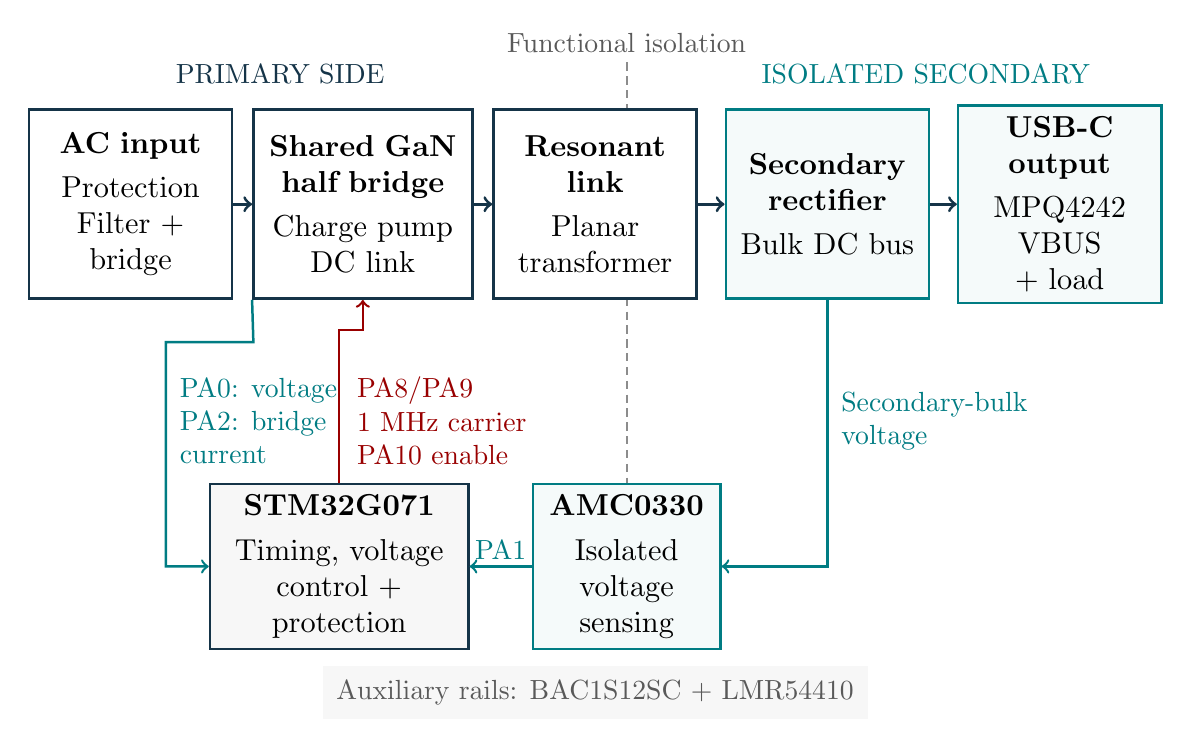
\begin{tikzpicture}[
    font=\fontsize{11}{13}\selectfont,
    block/.style={
        draw=reqNavy,fill=white,line width=0.9pt,
        text width=2.3cm,minimum height=2.4cm,
        align=center,inner sep=4pt,
        execute at begin node={\hyphenpenalty=10000\exhyphenpenalty=10000}
    },
    secondary/.style={block,draw=reqTeal,fill=reqTeal!4},
    controller/.style={
        block,text width=3.0cm,minimum height=1.5cm,fill=black!3
    },
    sensor/.style={
        block,draw=reqTeal,text width=2.1cm,
        minimum height=1.5cm,fill=reqTeal!4
    },
    powerflow/.style={->,draw=reqNavy,line width=1.1pt},
    feedback/.style={->,draw=reqTeal,line width=0.9pt},
    command/.style={->,draw=reqRed,line width=0.9pt},
    signaltext/.style={
        font=\fontsize{10}{12}\selectfont,
        text=reqTeal,fill=white,inner sep=2pt,align=left
    }
]
% Draw the functional boundary first so the transformer and isolated
% sensing blocks visibly span it rather than implying a bare-wire crossing.
\draw[densely dashed,draw=black!45,line width=0.8pt]
    (6.3,1.8) -- (6.3,-5.55);
\node[font=\fontsize{10}{12}\selectfont,text=reqNavy]
    at (1.9,1.65) {PRIMARY SIDE};
\node[font=\fontsize{10}{12}\selectfont,text=reqTeal]
    at (10.1,1.65) {ISOLATED SECONDARY};
\node[font=\fontsize{10}{12}\selectfont,text=black!65,
    fill=white,inner sep=2pt]
    at (6.3,2.05) {Functional isolation};

\node[block] (front) at (0,0)
    {\textbf{AC input}\\[3pt]Protection\\Filter + bridge};
\node[block,text width=2.5cm] (shared) at (2.95,0)
    {\textbf{Shared GaN}\\\textbf{half bridge}\\[3pt]Charge pump\\DC link};
\node[block] (link) at (5.9,0)
    {\textbf{Resonant}\\\textbf{link}\\[3pt]Planar\\transformer};
\node[secondary] (bulk) at (8.85,0)
    {\textbf{Secondary}\\\textbf{rectifier}\\[3pt]Bulk DC bus};
\node[secondary] (output) at (11.8,0)
    {\textbf{USB-C}\\\textbf{output}\\[3pt]MPQ4242\\VBUS + load};

\draw[powerflow] (front.east) -- (shared.west);
\draw[powerflow] (shared.east) -- (link.west);
\draw[powerflow] (link.east) -- (bulk.west);
\draw[powerflow] (bulk.east) -- (output.west);

\node[controller] (mcu) at (2.65,-4.6)
    {\textbf{STM32G071}\\[3pt]Timing, voltage\\control + protection};
\node[sensor] (sense) at (6.3,-4.6)
    {\textbf{AMC0330}\\[3pt]Isolated\\voltage sensing};

% Keep the primary-side acquisition route separate from carrier/enable
% commands and the isolated secondary-voltage feedback route.
\draw[feedback] (shared.south west)
    -- (1.56,-1.75) -- (0.45,-1.75)
    -- (0.45,-4.6) -- (mcu.west);
\node[signaltext,anchor=west] at (0.55,-2.75)
    {PA0: voltage\\PA2: bridge\\current};

\draw[command] (mcu.north)
    -- (2.65,-1.6) -- (2.95,-1.6) -- (shared.south);
\node[signaltext,text=reqRed,anchor=west] at (2.8,-2.75)
    {PA8/PA9\\1 MHz carrier\\PA10 enable};

\draw[feedback] (bulk.south) -- (8.85,-4.6) -- (sense.east);
\node[signaltext,anchor=west] at (8.95,-2.75)
    {Secondary-bulk\\voltage};
\draw[feedback] (sense.west) -- node[
    above,font=\fontsize{10}{12}\selectfont,
    text=reqTeal,inner sep=2pt] {PA1} (mcu.east);

\node[font=\fontsize{10}{12}\selectfont,text=black!65,
    fill=black!3,inner sep=5pt]
    at (5.9,-6.2) {Auxiliary rails: BAC1S12SC + LMR54410};
\end{tikzpicture}
\endgroup
\caption{Power and control architecture of the V1.0 prototype with the V1.1 circuit corrections. The transformer carries power across the isolation barrier, and the AMC0330 returns secondary-bulk feedback to the MCU. PA1 measures this feedback; PA0 and PA2 measure primary voltage and half-bridge current.}
\label{fig:req-hardware-architecture}
\end{figure}

\section{Operating States}
\label{sec:req-modes}

Startup, loaded regulation, and no-load energy limitation require distinct burst limits. The original prototype uses MCU pin PA10 as the active-high burst-enable output. UART provides command/status access, and ADC readings are buffered by DMA.

Table~\ref{tab:req-states} shows how the final firmware separates those tasks. Chapter~\ref{ch:control} gives the thresholds and timing behind the state changes.

\begin{table}[H]
\centering
\caption{States and options in the baseline firmware.}
\label{tab:req-states}
\begin{tabularx}{\textwidth}{@{}L{0.25\textwidth}Y@{}}
\toprule
State or option & Purpose and behavior\\
\midrule
Initialization & Configures stored settings, GPIO, UART, timers, ADC DMA, filters, and status indicators.\\
Off/inhibited & Holds PA10 low after an off command, reset condition, or latched fault.\\
Startup precharge & Applies limited bursts to power the secondary-side feedback circuit before normal regulation.\\
Open loop & Uses the commanded \texttt{OD} burst duty for bring-up and diagnostic operation.\\
Voltage control & Uses secondary-voltage thresholds and load-state logic to select bounded PA10 commands.\\
Loaded operation & Can hold the averaged \texttt{LDUTY} command and increase demand through \texttt{LBOOST} when secondary voltage falls.\\
No-load guard & Lowers the regulation window and caps the high command when the inferred load is high impedance.\\
Load-recovery override & Temporarily relaxes the no-load cap after a repeated low-voltage condition, allowing an attached load to receive power.\\
Line feed-forward & Uses PA0 to reduce the permitted high command as primary voltage rises; PA1 remains the feedback variable.\\
Fault latch & Inhibits PA10 until the cause is removed and the defined clear or reset action is performed.\\
\bottomrule
\end{tabularx}
\end{table}

The state logic changes permitted energy transfer while the active carrier remains at \SI{1}{\mega\hertz}. The burst envelope depends on load state and settings, including line feed-forward and \texttt{MAXRATE}. Precharge ends at either the readiness threshold or the configured attempt limit. The attempt limit can be reached before feedback becomes valid.

\section{Test and Design Checks}
\label{sec:req-matrix}

Tables~\ref{tab:req-functional-verification} and \ref{tab:req-performance-verification} list the tests and measurements needed to check each requirement.

\begin{table}[H]
\centering
\caption{Checks for the functional requirements.}
\label{tab:req-functional-verification}
\begin{tabularx}{\textwidth}{@{}L{0.10\textwidth}Y L{0.27\textwidth}@{}}
\toprule
ID & Test or measurement & Results section\\
\midrule
FR-01 & Startup sequence, output rise, and transition to valid feedback & \cref{sec:res-startup}\\
FR-02 & Carrier frequency and enable timing & \cref{sec:res-bringup}\\
FR-03 & Secondary and connector voltage under load & \cref{sec:res-steady}\\
FR-04 & No-load and load-removal response & \cref{sec:res-open}\\
FR-05 & Applied load step, voltage excursion, and recovery & \cref{sec:res-transient}\\
FR-06 & Enabled OVP threshold, inhibit action, and fault recovery & \cref{sec:res-open,sec:res-fwcompare}\\
FR-07 & DMA and loop-timing implementation & \cref{sec:res-fwcompare}\\
FR-08 & Command, configuration, and status access & \cref{sec:res-fwcompare}\\
\bottomrule
\end{tabularx}
\end{table}

\begin{table}[H]
\centering
\caption{Checks for the performance requirements.}
\label{tab:req-performance-verification}
\begin{tabularx}{\textwidth}{@{}L{0.10\textwidth}Y L{0.27\textwidth}@{}}
\toprule
ID & Test or measurement & Results section\\
\midrule
PR-01 & Measured power together with available duration and thermal record & \cref{sec:res-steady,sec:res-thermal}\\
PR-02 & Stated source voltage and frequency & \cref{sec:res-steady}\\
PR-03 & Selected output mode, load, and measured VBUS & \cref{sec:res-bringup,sec:res-steady}\\
PR-04 & DC voltage, ripple capture, and load response & \cref{sec:res-steady,sec:res-transient}\\
PR-05 & No-load voltage observations and control thresholds & \cref{sec:res-open}\\
PR-06 & Corresponding power, PF, and current-distortion record & \cref{sec:res-pq}\\
PR-07 & Input/output power measured under the same conditions and at stated circuit points & \cref{sec:res-efficiency}\\
PR-08 & Surface-temperature record and operating condition & \cref{sec:res-thermal}\\
PR-09 & Hardware, firmware, and source measurements for each result & \cref{sec:res-compliance}\\
PR-10 & Active limiter and observed overload response & \cref{sec:res-transient,sec:res-compliance}\\
\bottomrule
\end{tabularx}
\end{table}

Section~\ref{sec:res-compliance} compares requirements with completed measurements; Section~\ref{sec:revised-plan-criteria} extends the scope to V2/V3 development. Source code shows which functions were implemented; measurements show how the circuit responded.

\section{Requirements from the Revised Plan}
\label{sec:revised-plan-criteria}

The revised July--October plan extends bring-up into V2 evaluation, converter adjustment, and V3 edge-card development \cite{projectOctoberPlan}. The plan calls for repeating the V2 tests, finding the output-power limit, testing controlled design changes, and preparing the final evaluation.

\Needspace{10\baselineskip}
\subsection{Power Levels and Prototype Versions}

The revised plan sets \SI{65}{\watt} continuous output as the minimum and \SI{100}{\watt} continuous output as the target. The earlier plan schedules \SI{75}{\watt} continuous validation as an intermediate test milestone \cite{projectEarlierPlan}. Each continuous level requires a defined run time, stated ambient and cooling conditions, stable electrical operation, and a temperature record over the run.

The plan calls for a repeat of the reported V2 maximum near \SI{85}{\watt} under defined conditions, or an explanation of the difference. The integrated MCU and its ported firmware form part of the V2 development described in Sections~\ref{sec:hw-v2} and \ref{sec:ctrl-pwr2-port}. The separate matched measurements on the modified V1.0 assembly reached \SI{79.89}{\watt}.

\subsection{Design and Test Requirements}

Table~\ref{tab:req-revised-plan-criteria} lists the additional design work and tests, including temperature, stability, and volume measurements.

\begingroup
\small
\begin{longtable}{@{}L{0.10\linewidth}L{0.82\linewidth}@{}}
\caption[Tests and design work in the revised plan.]{Tests and design work in the revised project plan.}
\label{tab:req-revised-plan-criteria}\\
\toprule ID & Planned test or design work\\\midrule
\endfirsthead
\toprule ID & Planned test or design work\\\midrule
\endhead
AP-01 & Assess the \SI{65}{\watt} continuous minimum, earlier \SI{75}{\watt} validation milestone, and \SI{100}{\watt} continuous target using simultaneous electrical measurements and defined-duration thermal and stability runs.\\
AP-02 & Repeat the reported approximately \SI{85}{\watt} V2 point, or explain the difference. State the assembly and fitted parts, firmware settings, input/output conditions, instrument and probe settings, ambient, cooling, duration, and uncertainty.\\
AP-03 & Diagnose the \SI{15}{\watt} reported output shortfall using loss calculations, component stress, control limits, and temperatures. Rank candidate changes from these findings and retest one change at a time. If \SI{100}{\watt} is not reached safely, quantify the highest repeatable power and the remaining limit.\\
AP-04 & Characterize no load, the supported fixed PDOs, and PPS. At applicable loads, record regulation, corresponding input/output power, efficiency, PF/THD, ripple, switching/device stress, transient response, temperatures, and protection events. The planned V2 points include \SIlist{25;45;65;75;80}{\watt} and approximately \SI{85}{\watt}.\\
AP-05 & Complete a defined-duration thermal and stability run at the final supported power and document extended-load reliability observations. State ambient, cooling, run time, temperature development, interruptions, and stop limits.\\
AP-06 & Develop and review the V3 edge-card pinout, outline, component-height limit, current and gate/sense return paths, creepage/clearance, and thermal-spreading arrangement. Record schematic/layout review, DRC, BOM availability, manufacturing review, and release status.\\
AP-07 & Compare V2 and V3 power density using the same volume calculation and output-power test conditions. Report dimensions, included parts and cooling allowance, efficiency, thermal margin, and any safety or reliability trade-off.\\
AP-08 & Determine whether V3 is ready for testing, identify the tests that can be completed, and state the remaining work. If V3 is not ready, use the completed V2 tests with matched operating conditions as the hardware results.\\
\bottomrule
\end{longtable}
\endgroup

\subsection{Power Density and Remaining Work}

Power density requires verified output and complete assembly dimensions. Section~\ref{sec:method-density} uses a common rectangular envelope including magnetics, connectors, supports, component height, required spacing, and cooling hardware. V2 and V3 assembly dimensions remain necessary; they cannot be inferred from the V1.0 outline.

The completed work includes the measured first-prototype baseline, integrated V2 circuit and firmware, powered tank changes, and a reduced V3 layout. Replacement planar magnetics were not installed. A matched repeat near \SI{85}{\watt}, the full PPS and extended-load tests, a decision on V3 testing, and the full-system power-density comparison remain open. Chapter~\ref{ch:results} presents the measurements and design estimate; Chapters~\ref{ch:discussion} and \ref{ch:conclusion} connect them to the next steps.

Planar-magnetic optimization is a learning objective. The supplied designs were retained, so this thesis evaluates their integration and effect on converter operation. The original electromagnetic design came from the earlier work described in Section~\ref{sec:intro-contributions}.

